\begin{apendicesenv}
\chapter{BER vs SNR}

Com base na implementação do receptor e transmissor apresentada nas seções \ref{sec:receptor} e \ref{sec:transmissor}, foi realizado um estudo de desempenho do sistema, variando a relação \gls{EbN0} e medindo a \gls{BER} para cada valor, comparando o desempenho do sistema ARGOS-3 com modulação \gls{QPSK} (tanto teórica quanto simulada), conforme apresentado na \autoref{fig:ber_snr}.

\begin{figure}[H]
	\centering
	\caption{Comparação BER vs SNR - ARGOS3 e QPSK}\label{fig:ber_snr}
	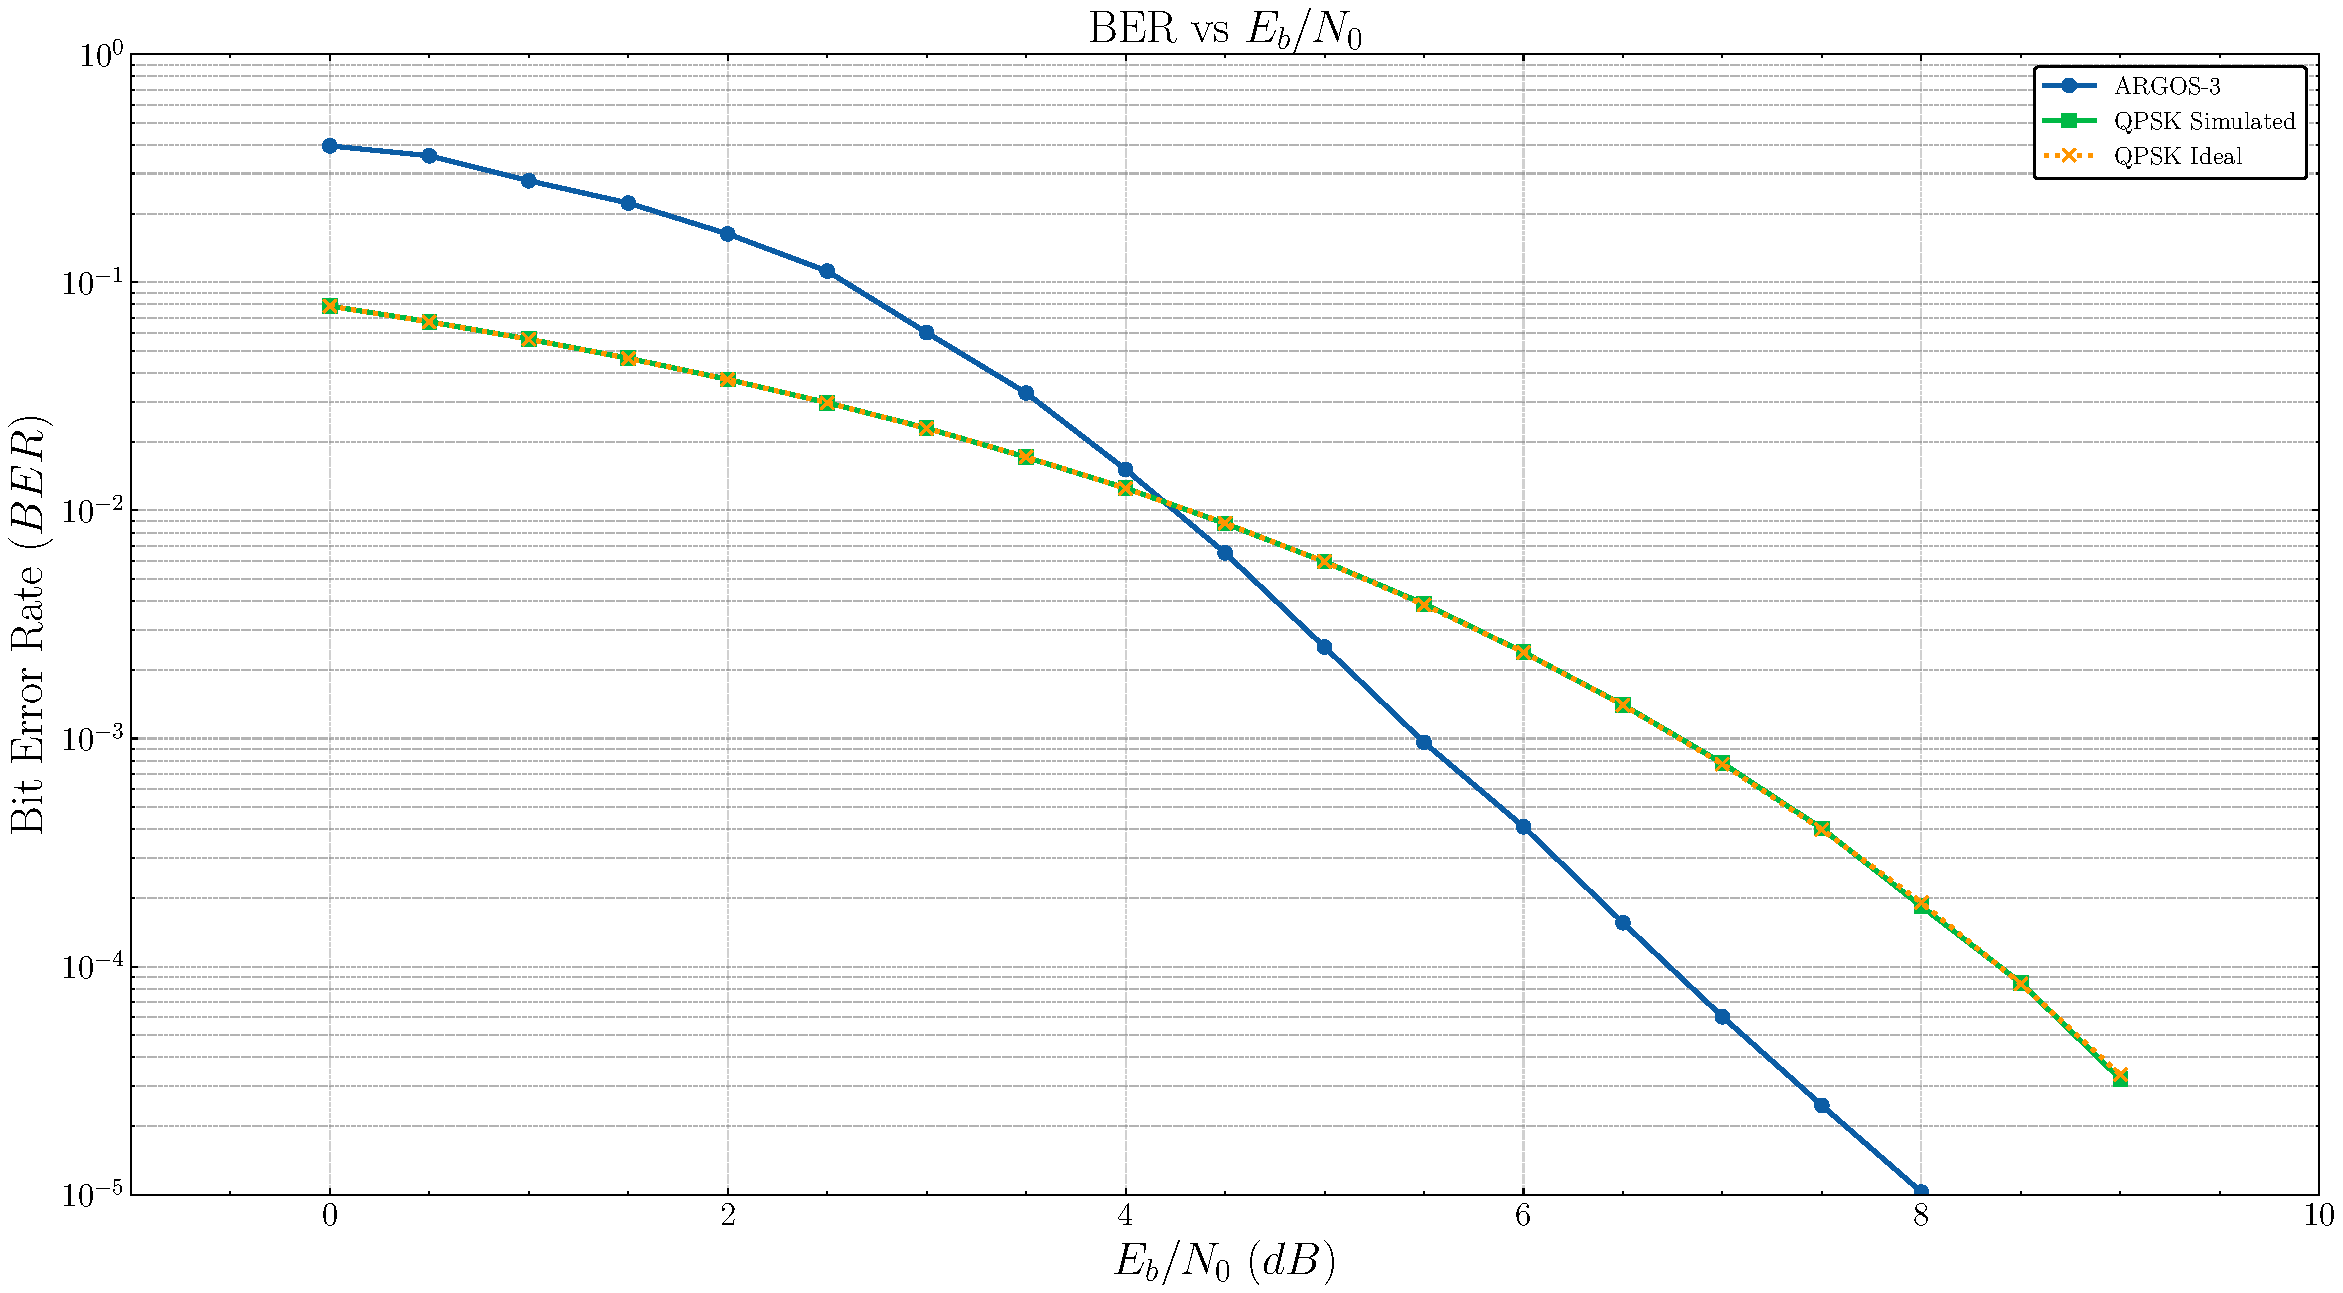
\includegraphics[width=\linewidth]{assets/apendice/ber_vs_ebn0.pdf}
\end{figure}

Nota-se que o desempenho do sistema ARGOS-3 está melhor do que o desempenho teórico e simulado da modulação \gls{QPSK} pura, o que pode ser explicado pela presença do código convolucional, que adiciona redundância aos dados transmitidos, permitindo a correção de erros no receptor, além da presença da técnica de codificação de linha \gls{Manchester}, que também contribui para a melhoria das características do sinal modulado.

\end{apendicesenv}
